\documentclass[12pt, letterpaper]{article}

\usepackage[a4paper,left=2.5cm,right=2cm,top=2.5cm,bottom=2.5cm]{geometry}
\usepackage[utf8x]{inputenc}
\usepackage[german]{babel}
\usepackage{graphicx}
\usepackage{caption}
\usepackage{minted} %code
\usepackage{amsmath}
\usepackage[colorinlistoftodos]{todonotes}
\usepackage{fancyhdr}
\usepackage{hyperref}
\usepackage{mathpazo} % Palatino font
\usepackage{float}


\hypersetup{
    colorlinks,
    citecolor=black,
    filecolor=black,
    linkcolor=black,
    urlcolor=black
}

\pagestyle{fancy}
\fancyhf{}
\rhead{Daniel Englisch}
\lhead{WEA5-Wetr}
\rfoot{\thepage}
 
\setminted[]{
	frame=single,
	breaklines,
	samepage=false
} 

\usemintedstyle{csharp}

\graphicspath{ {pictures/} }

%----------------------------------------------------------------------------------------
% COMMANDS
%----------------------------------------------------------------------------------------

\newcommand{\img}[3] {
\begin{figure}[H]
	\centering
	\includegraphics[width=#3\linewidth]{#1}
	\caption{#2}
\end{figure}
}

 
%----------------------------------------------------------------------------------------
% BEGIN
%----------------------------------------------------------------------------------------

\begin{document}

%----------------------------------------------------------------------------------------
%	TITLE PAGE
%----------------------------------------------------------------------------------------

\begin{titlepage} % Suppresses displaying the page number on the title page and the subsequent page counts as page 1
\newcommand{\HRule}{\rule{\linewidth}{0.5mm}} % Defines a new command for the horizontal lines, change thickness here

\center % Center everything on the page
 
%----------------------------------------------------------------------------------------
%	HEADING SECTIONS
%----------------------------------------------------------------------------------------

\textsc{\LARGE FH Hagenberg}\\[1.5cm] % Name of your university/college
\textsc{\Large Projektarbeit}\\[0.5cm] % Major heading such as course name
%\textsc{\large Minor Heading}\\[0.5cm] % Minor heading such as course title

%----------------------------------------------------------------------------------------
%	TITLE SECTION
%----------------------------------------------------------------------------------------

\HRule \\[0.4cm]
{ \huge \bfseries Weather Tracer - Dokumentation}\\[0.4cm] % Title of your document
\HRule \\[1.5cm]


\begin{minipage}{0.9\textwidth}
\begin{flushleft} \large
\emph{Autor:}\\
Daniel \textsc{Englisch}\\
\end{flushleft}
\end{minipage}

\begin{minipage}{0.9\textwidth}
\begin{flushright} \large
\emph{Übungsleiter:} \\
Stefan \textsc{Nadschläger} % Supervisor's Name
\end{flushright}
\end{minipage}\\[2cm]


{\large \today}\\[1cm] 
{Angular Application}\\[2cm]



\includegraphics[scale=0.15]{img/logo.png}
 

\vfill 
\end{titlepage}


\tableofcontents
\newpage

\setlength\parindent{0pt}


\section{Inbetriebnahme}

Um das Wetr-Frontend in Betrieb zu nehmen, muss die aktuellste Version von GitHub\footnote{https://github.com/DanielEnglisch/wetr-frontend} heruntergeladen werden. Hierfür müssen zuvor folgende Pakete installiert werden:
\begin{itemize}
    \item Yarn\footnote{https://yarnpkg.com/en/docs/install}
    \item windows-build-tools (\textit{yarn add g windows-build-tools})
    \item karma-cli (\textit{yarn add g karma-cli})
    \item angular-cli (\textit{yarn add g @angular/cli@6.1.3})
\end{itemize}

Natürlich müssen die in der \textit{package.json} Datei spezifizierten Pakete installiert werden mit \textit{yarn install --check-files}.  Um die Applikation zu bauen und bereitzustellen muss im Projektverzeichnis der Befehl \textit{ng server --port 80} ausgeführt werden.\\

Danach kann die Applikation unter \textit{http://localhost/} aufgerufen werden.
Beachten Sie, dass für die fehlerfreie Verwendung die Wetr-RestAPI unter dem Port $5000$ bereits laufen muss. Falls diese API unter einer anderen \textit{Host:Port}-Kombination erreichbar ist, kann dies in der Datei \textit{src/app/services/api.servive.ts} bei der Konstanten 'apiString' angepasst werden.
\newpage

\section{Aufbau}

Im Projekt existieren folgende \textbf{Services}:
\begin{itemize}
    \item \textbf{ApiService} - Zuständig für die Kommunikation mit der Wetr-RestAPI.
    \item \textbf{SettingsService} - Für das Speichern und Lesen der Benutzereinstellungen im \textit{localStorage} verantwortlich.
\end{itemize}

Weiters existieren folgende \textbf{Komponenten} welche in Abschnitt \ref{components} genauer beschrieben werden:
\begin{itemize}
    \item \textbf{App} - Hauptkomponente die unter anderem die Navigationsleiste beinhaltet.
    \item \textbf{Login} - Zum Eingeben der Zugangsdaten zur Wetr-Plattform.
    \item \textbf{Home} - Zeigt eine Übersicht über die eigenen Stationnen an.
    \item \textbf{StationCard} - Wiederverwendbare Komponente die eine Station repräsentiert.
    \item \textbf{EditStation} - Formular zum Editieren einer Station.
    \item \textbf{AddStation} - Formular zum Hinzufügen einer Station.
    \item \textbf{Search} - Zum Suchen von Stationen in Communities.
    \item \textbf{Query} - Um Daten einer Station abzufragen und neue Messwerte einzufügen.
    \item \textbf{Dashboard} - Zum anzeigen von favorisierten Stationsabfragen pro Benutzer.
    \item \textbf{DashboardCard} - Wiederverwendbare Komponente zum grafischen Darstellen einer gespeicherten Abfrage.
    \item \textbf{Settings} - Lokale Seite zum Ändern von Einstellungen.

\end{itemize}

\textbf{Verwendete externe Pakete}:\\
\textit{Angular Material, Bootstrap 4, FlashMessages, hightCharts, ng-datetime-picker, fontawesome-icons, ...}


\newpage

\section{Details: ApiService}
\label{components}

Der \textit{ApiService} wurde nicht mit \textit{Swagger} generiert, sondern selbst geschrieben, um ein besseres Verständnis für die Funktionsweise solche einer Architektur zu erlangen.\\

Beim erstmaligen Starten der Applikation wird überprüft, ob sich ein Token im localStorage befindet. Falls nicht, wird der Benutzer aufgefordert sich einzuloggen. Beim Einloggen wird ein normaler Post-Request zur API gesendet und bei Erfolg der Token für abgesicherte Routen zurückgegeben. Diese wird im localStorage gespeichert.\\

Für Anfragen auf gesicherte Routen wird ein Art Wrapper für Get/Post/Put/Delete-Requests verwendet, der als Auth-Header den vorher erwähnten Token mitsendet. Für Anfragen, die dies nicht benütigen werden die normalen von der Angular-Klasse \textit{HttpClient} zur Verfügung gestellten Methoden verwendet.\\

Falls der Token abgelaufen ist, wird der Status Code 401 empfangen und zur Login-Seite umgeleitet um nach erneutem Einloggen einen neuer Token zu erhalten.\\

Zuständigkeiten der ApiService Klasse:
\begin{itemize}
    \item \textbf{Statische Daten}
        \begin{itemize}
            \item \textit{loadStaticData()} - Einmaliges Anfordern von statischen Daten wie StationTypes oder Communitier.
            \item \textit{revolve...()} - Auflösen einer Id zu der Bezeichnung.
            \item \textit{get...()} - Rückgabe des angeforderten Arrays.
        \end{itemize}
    \item \textbf{Login}
    \begin{itemize}
        \item \textit{login()} - Anfordern eines Tokens.
        \item \textit{getEmail()} - Liefert die E-Mail-Addresse des eingeloggten Benutzers.
        \item \textit{loggedIn()} - Ob gerade ein Benutzer eingeloggt ist.
        \item \textit{logout()} - Löschen des Tokens.
    \end{itemize}
    \item \textbf{Dashboard\footnote{Für jeden eingeloggten Benutzer individuell.}}
    \begin{itemize}
        \item \textit{getDashboardQueries()} - Laden der im localStorage sich befindenden DashboardQueries pro Benutzer.
        \item \textit{addQueryToDashboard()} - Hinzufügen neuer DashboardQueries für den aktuellen Benutzer.
        \item \textit{removeQueryToDashboard()} - Löschen eines DashboardQueries für den aktuellen Benutzer.
    \end{itemize}
    \newpage
    
    \item \textbf{Local Storage}
    \begin{itemize}
        \item \textit{loadLocalStorage()} - Laden der für diese Applikation relevanten localStorage-Daten.
        \item \textit{saveLocalStorage()} - Speichern der für diese Applikation relevanten localStorage-Daten.
    \end{itemize}
    
    \item \textbf{Http Communication}
    \begin{itemize}
        \item \textit{Jwt[VERB]()} - Authentifizierte Anfrage an die RestAPI.
        \item \textit{[VERB]()} - Anonyme Anfrage an die RestAPI.
    \end{itemize}
    
    \item \textbf{Stations}
    \begin{itemize}
        \item \textit{getMyStations()} - Liefert die Stationen des eingeloggten Benutzers.
        \item \textit{getStation(id)} - Liefert die Station mit der eingebenden Id.
        \item \textit{getStationsForCommunity()} - Liefert alle Stationen für die eine Community.
        \item \textit{deleteStation()} - Löscht eine Station des eingeloggten Benutzers.
        \item \textit{editStatoin()} - Bearbeitet eine Station des eingeloggten Benutzers.
         \item \textit{addStation()} - Fügt eine neue Station für den eingeloggten Benutzer hinzu.
        \item \textit{queryStation()} - Fragt Messdaten für die gewüschte Station ab.
        \item \textit{addMeasurement()} - Fügt einer Station neue Messdaten hinzu.

    \end{itemize}
\end{itemize}



\newpage
\section{Komponenten}

\subsection{App}

Diese Hauptkomponente wird als Template für alle anderen Seiten verwendet.
Sie beinhaltet die Navbar mit der auf alle anderen Komponenten dieser Applikation navigiert werden kann. Im eingeloggten Zustand werden alle möglichen Navigationsbutton angezeigt (Abbildung \ref{fig:navbar_loggedIn}). Beim ausgeloggten Zustand wird nur der Button zur öffentlichen Suche und zum Einloggen angezeigt (Abbildung \ref{fig:navbar_loggedOut}).

\begin{figure}[H]
    \centering
    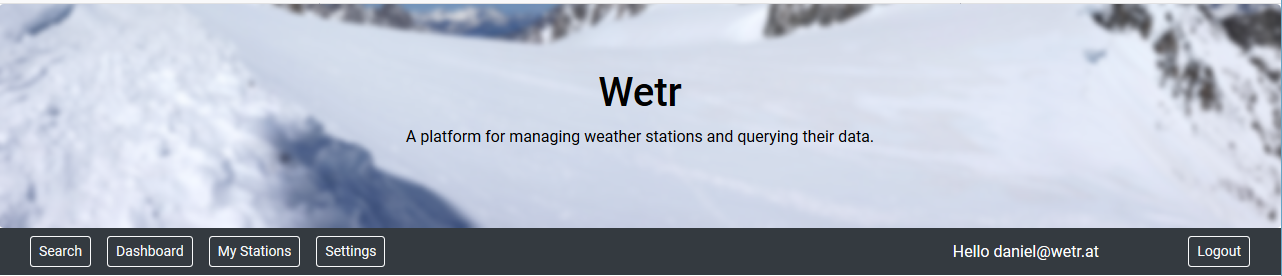
\includegraphics[width=\textwidth]{img/app/navbar.png}
    \caption{Gleichbleibender Inhalt der Seite mit Navbar im eingeloggten Zustand.}
    \label{fig:navbar_loggedIn}
\end{figure}


\begin{figure}[H]
    \centering
    
\includegraphics[width=\textwidth]{img/app/navbar_loggedOut.png}
    \caption{Navbar im ausgeloggtem Zustand.}
    \label{fig:navbar_loggedOut}
\end{figure}


\subsection{Login}

Die Login-Seite beinhaltet zwei Felder zum Eingaben der Benutzerdaten, welche live validiert werden. Nur wenn die Daten valide sind, kann der Login-Button gedrückt werden (Abbildung \ref{fig:login_page}). Während der API-Abfrage wird ein Ladeindikator angezeigt. Solch ein Indikator wird in der gesamten Applikation bei ledenden Elementen angezeigt und wird dahen nicht länger erwähnt. Bei falschen Zugangsdaten wird ein entsprechender Fehler angezeigt  (Abbildung \ref{fig:invalid_login}).


\begin{figure}[H]
    \centering
    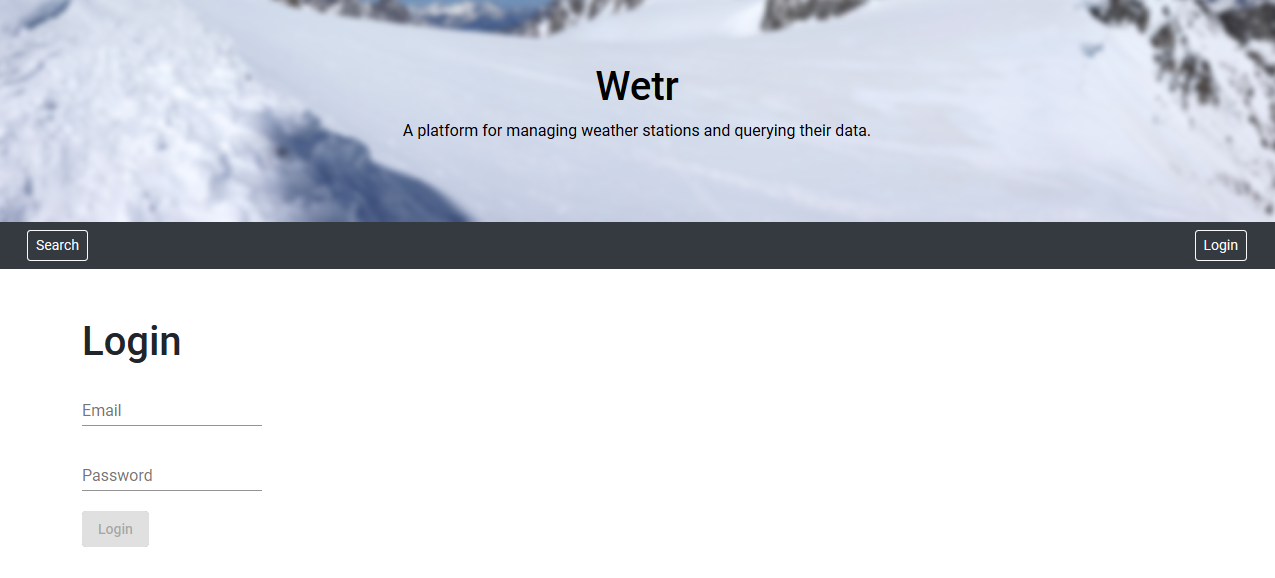
\includegraphics[width=\textwidth]{img/login/login.png}
    \caption{Die Login-Seite.}
    \label{fig:login_page}
\end{figure}


\begin{figure}[H]
    \centering
    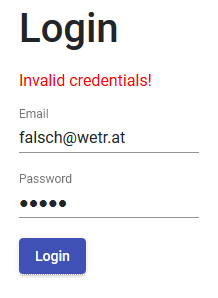
\includegraphics[scale=1.0]{img/login/invalid.png}
    \caption{Login-Seite mit falschen Zugangsdaten.}
    \label{fig:invalid_login}
\end{figure}


\subsection{Home}

Nach dem erfolgreichen Einloggen werden die Stationen des eingeloggten Benutzers angezeigt (Abbildung \ref{fig:myStations}). Es ist hier möglich Details zu den angezeigten Stationen auszublenden und neue Stationen anzulegen (siehe Abschnitt \ref{addStation}). Die Details zu den angezeigten StationCards wird in Abschnitt \ref{stationcards} beschrieben.

\begin{figure}[H]
    \centering
    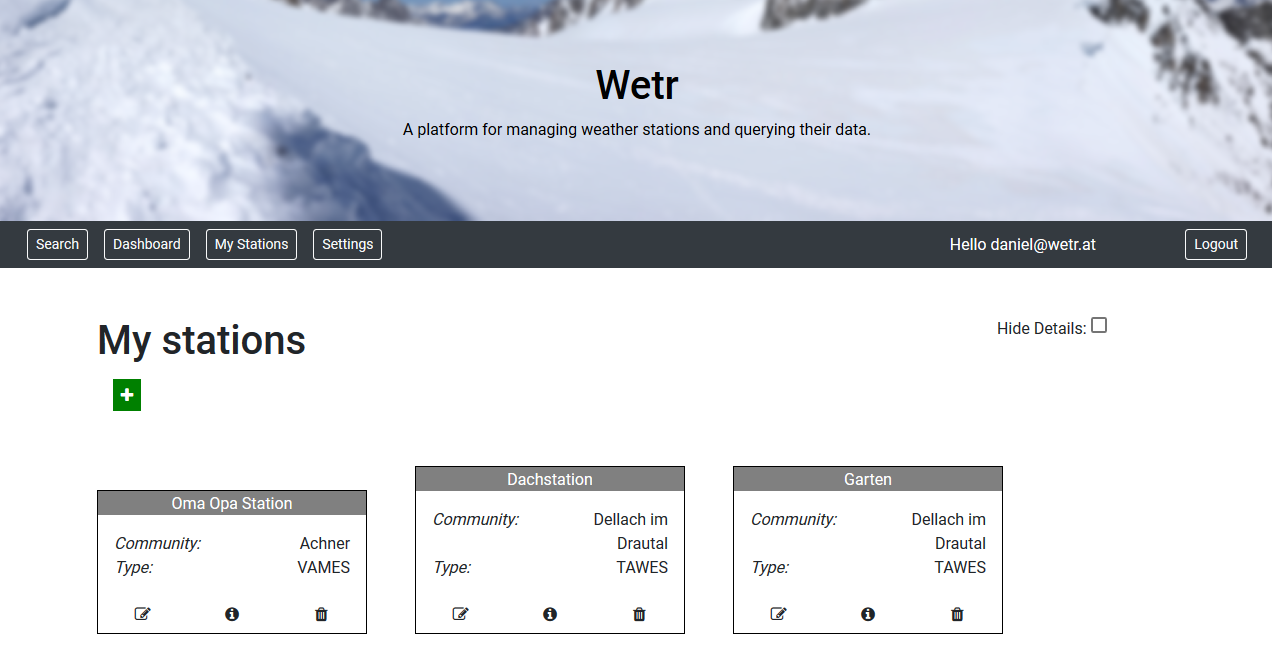
\includegraphics[width=\textwidth]{img/stations/mystations.png}
    \caption{Übersicht über die Stationen des eingeloggten Benutzers.}
    \label{fig:myStations}
\end{figure}

\newpage
\subsection{StationCard}
\label{stationcards}

Diese Komponente repräsentiert die Anzeige einer Station. Es gibt vier verschiedene Ansichten der StationCards:
\begin{itemize}
    \item Ansicht: MyStations, detailreich - Abbildung \ref{fig:stations_detail}
    \item Ansicht: MyStations - Abbildung \ref{fig:stations_normal}
    \item Ansicht: Search, detailreich - Abbildung \ref{fig:search_detail}
    \item Ansicht: Search - Abbildung \ref{fig:search_normal}
\end{itemize}

Die öffentliche suche wird in Abschnitt \ref{search} beschrieben.

\begin{figure}[H]
    \centering
    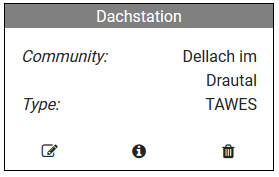
\includegraphics[scale=1.0]{img/stations/stations_detail.png}
    \caption{StationCard in der Detailansicht mit der Möglichkeit zum Abfragen, Bearbeiten und Löschen.}
    \label{fig:stations_detail}
\end{figure}

\begin{figure}[H]
    \centering
    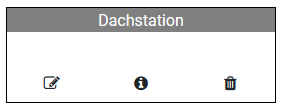
\includegraphics[scale=1.0]{img/stations/stations.png}
    \caption{StationCard in der reduzierten Ansicht mit der Möglichkeit zum Abfragen, Bearbeiten und Löschen.}
    \label{fig:stations_normal}
\end{figure}

\begin{figure}[H]
    \centering
    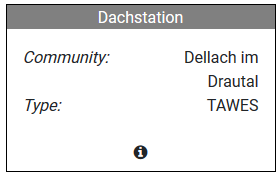
\includegraphics[scale=1.0]{img/stations/search_detail.png}
    \caption{StationCard in der Detailansicht mit der Möglichkeit zum Abfragen.}
    \label{fig:search_detail}
\end{figure}

\begin{figure}[H]
    \centering
    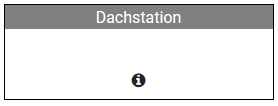
\includegraphics[scale=1.0]{img/stations/search.png}
    \caption{StationCard in der reduzierten Ansicht mit der Möglichkeit zum Abfragen.}
    \label{fig:search_normal}
\end{figure}
\newpage


\subsection{EditStation}
\label{editStation}
Ansicht zum Editieren von Stationen (Abbildung \ref{fig:editStation}). Es können nur eigene Stationen editiert werden. Das Formular kann nur abgeschickt werden, wenn es valide ist. Beim Erfolgreichen Ändern der Daten bzw. bei Fehlern wird eine entsprechende FlashMessage angezeigt (Abbildung \ref{fig:editStation_success}). Dies ist im gesamten System gleich und wird daher nicht länger durch Screenshots gezeigt.

\begin{figure}[H]
    \centering
    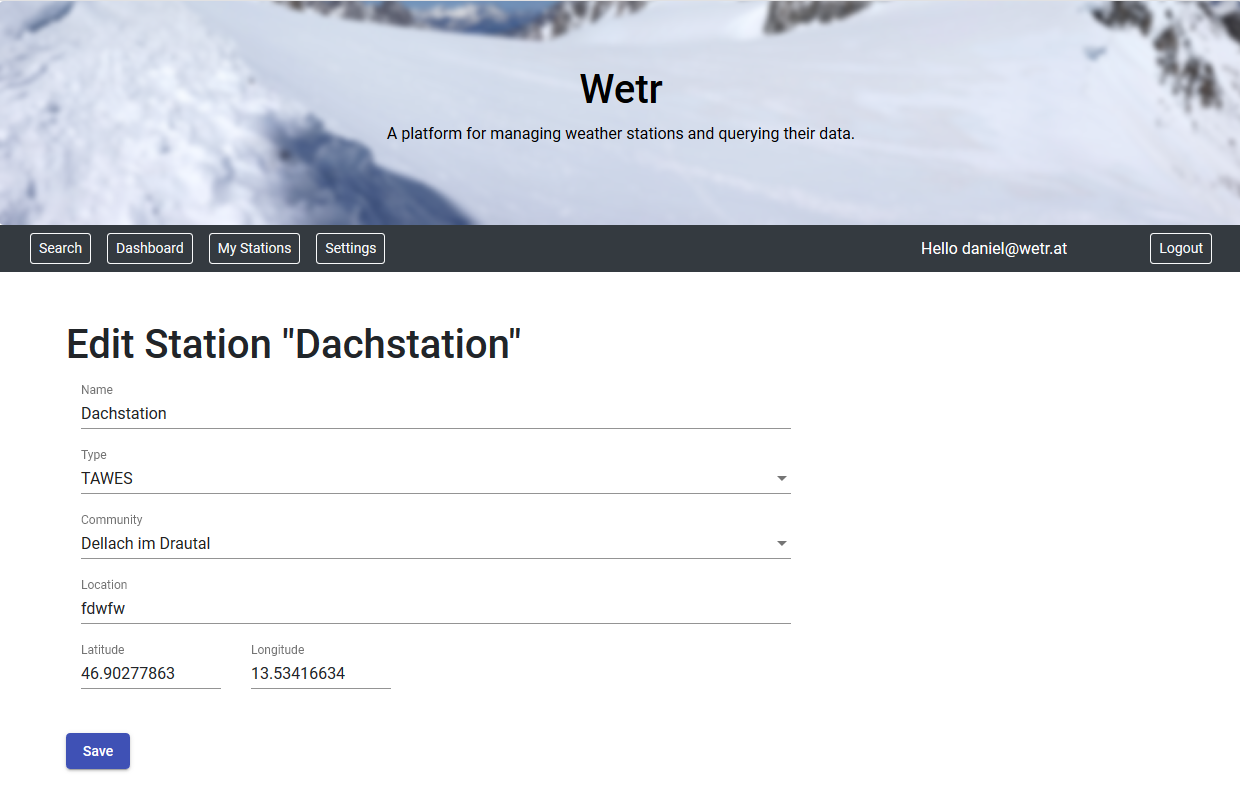
\includegraphics[width=\textwidth]{img/edit/edit_station.png}
    \caption{Formular zum Bearbeiten von Stationsdaten.}
    \label{fig:editStation}
\end{figure}

\begin{figure}[H]
    \centering
    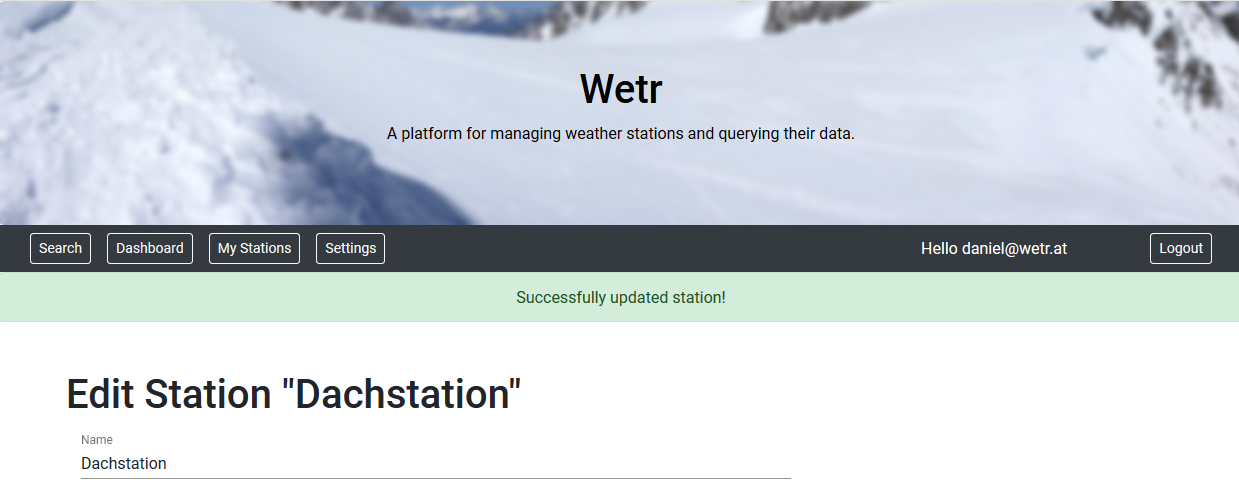
\includegraphics[width=\textwidth]{img/edit/edit_success.png}
    \caption{Anzeige von FlashMessages in dieser Applikation.}
    \label{fig:editStation_success}
\end{figure}
\newpage

\subsection{AddStation}
\label{addStation}

Die Funktionsweise und das Aussehen sind sehr ähnlich zum Editieren einer Station (Abschnitt \ref{editStation}), deshalb werden hier keine Screenshots gezeigt.

\subsection{Search}
\label{search}

Auf dieser Seite kann nach Stationen gesucht werden (Abbildung \ref{fig:search_nothing}).
Die Eingabe der Community wird durch autocompletion unterstützt (Abbildung \ref{fig:search_autocomplete}).
Die Ergebnisse der Suche werden mit StationCard-Komponenten angezeigt (Abbildung \ref{fig:search_results}). Hierbei können die Details zu einer Station wieder versteckt werden.

\begin{figure}[H]
    \centering
    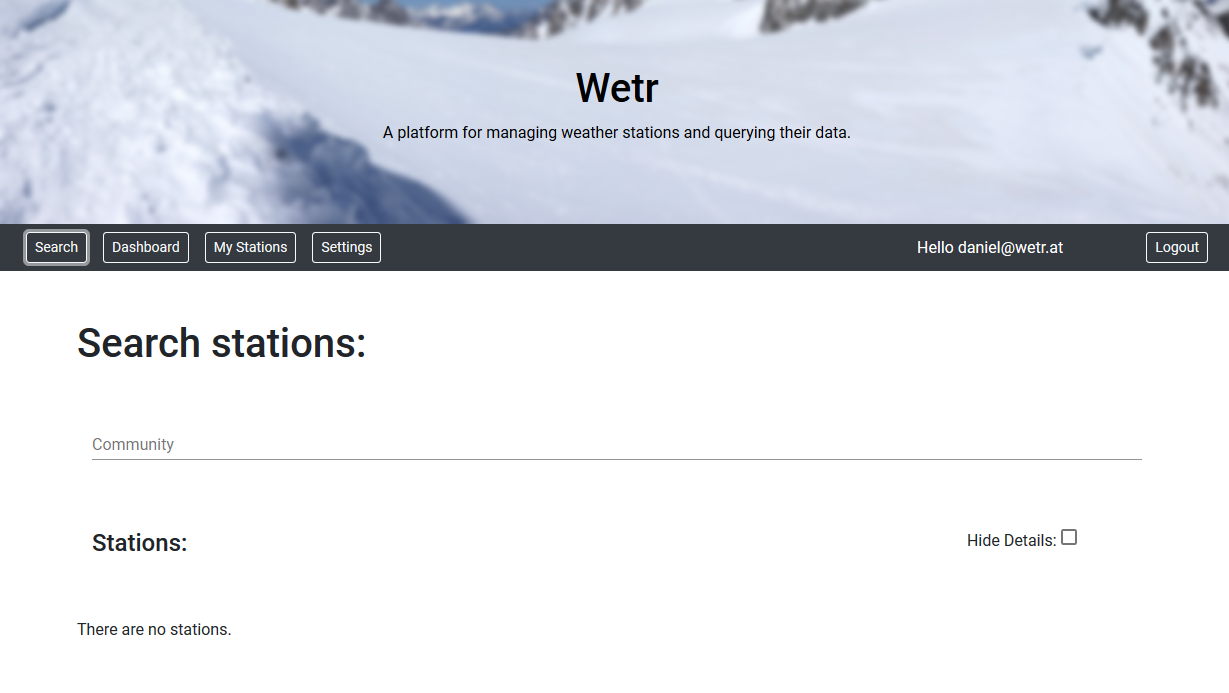
\includegraphics[width=\textwidth]{img/search/search_nothing.png}
    \caption{Übersicht der öffentlichen Suche ohne Ergebnisse.}
    \label{fig:search_nothing}
\end{figure}


\begin{figure}[H]
    \centering
    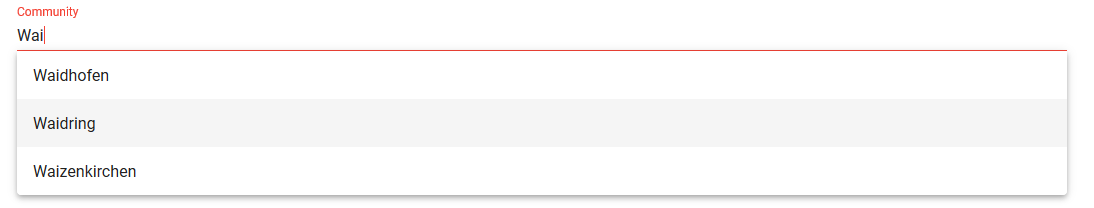
\includegraphics[width=\textwidth]{img/search/search_autocomplete.png}
    \caption{Darstellung der AutoCompletion bei Communities.}
    \label{fig:search_autocomplete}
\end{figure}

\begin{figure}[H]
    \centering
    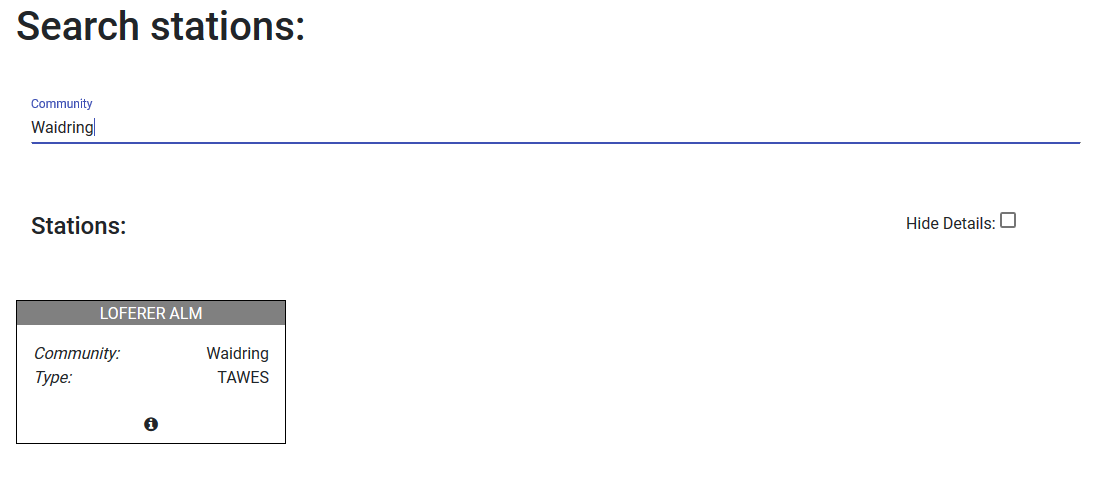
\includegraphics[width=\textwidth]{img/search/search_results.png}
    \caption{Resultate einer öffentlichen Suche.}
    \label{fig:search_results}
\end{figure}


\subsection{Query}

Auf dieser Seite können einerseits Abfragen zu Messdaten gemacht werden bzw. diese angelegt werden (Abbildung \ref{fig:query_form}). Das linke Formular beinhaltet zur Auswahl der Start und Enddatums der Abfrage einen Datpicker (Abbildung \ref{fig:query_datepicker}). Die Dropdowns sind mit den möglichen Abfragekriterien bestückt. Das Ergebnis der Abfrage wird unten in einem Chart (Abbildung \ref{fig:query_chart}) und in tabellarischer Form (Abbildung \ref{fig:query_table}) dargestellt. Beim Einfügen von Messdaten wird zur Eingabe der Timestamp ein DateTime Picker verwendet (Abbildung \ref{fig:query_datetime}).
Es können Abfragen zum Dashboard hinzugefügt werden, wobei diese als Enddatum das heutige Datum haben müssen um beispielsweise eine Abfrage zu ermöglichen, die die Durchschnittstemperatur der letzten zwei Wochen anzeigt.

\begin{figure}[H]
    \centering
    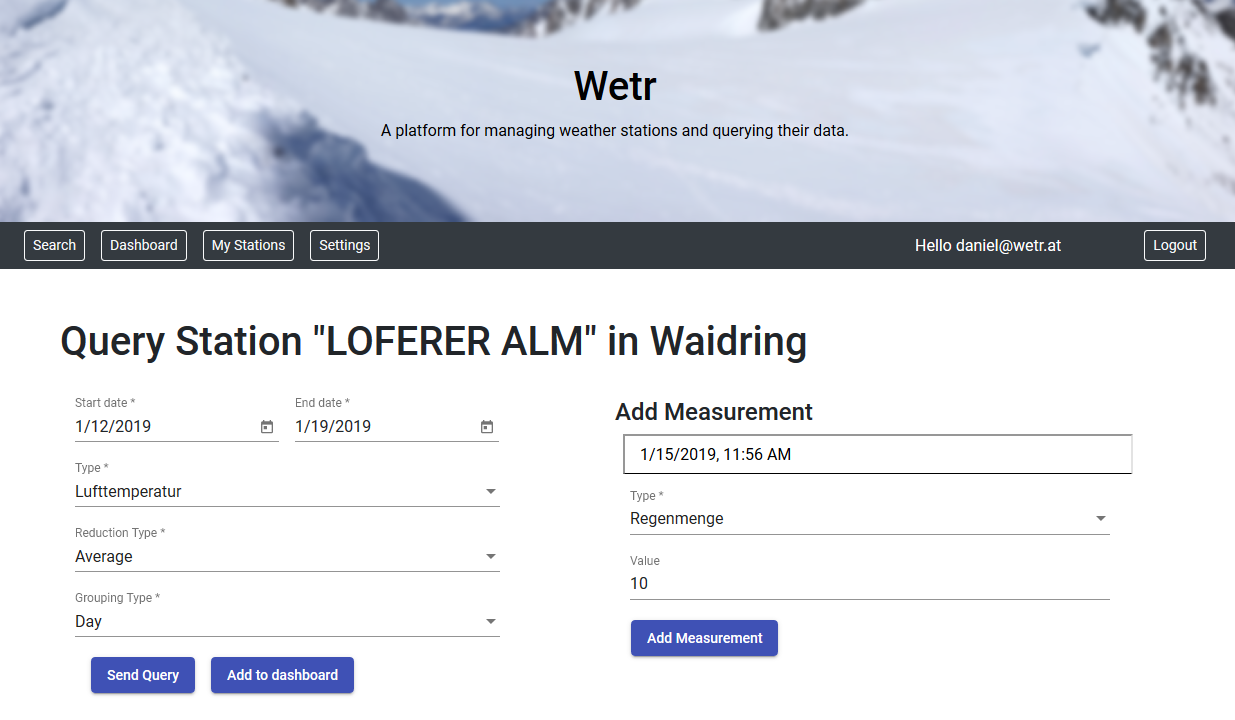
\includegraphics[width=\textwidth]{img/query/query_form.png}
    \caption{Formular zum Abfragen und Hinzufügen von Messdaten.}
    \label{fig:query_form}
\end{figure}

\begin{figure}[H]
    \centering
    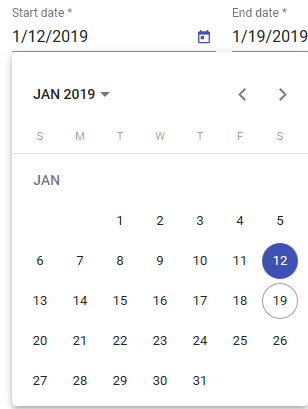
\includegraphics[scale=1.0]{img/query/query_date.png}
    \caption{DatePicker für Start und Enddatum bei Abfragen.}
    \label{fig:query_datepicker}
\end{figure}

\begin{figure}[H]
    \centering
    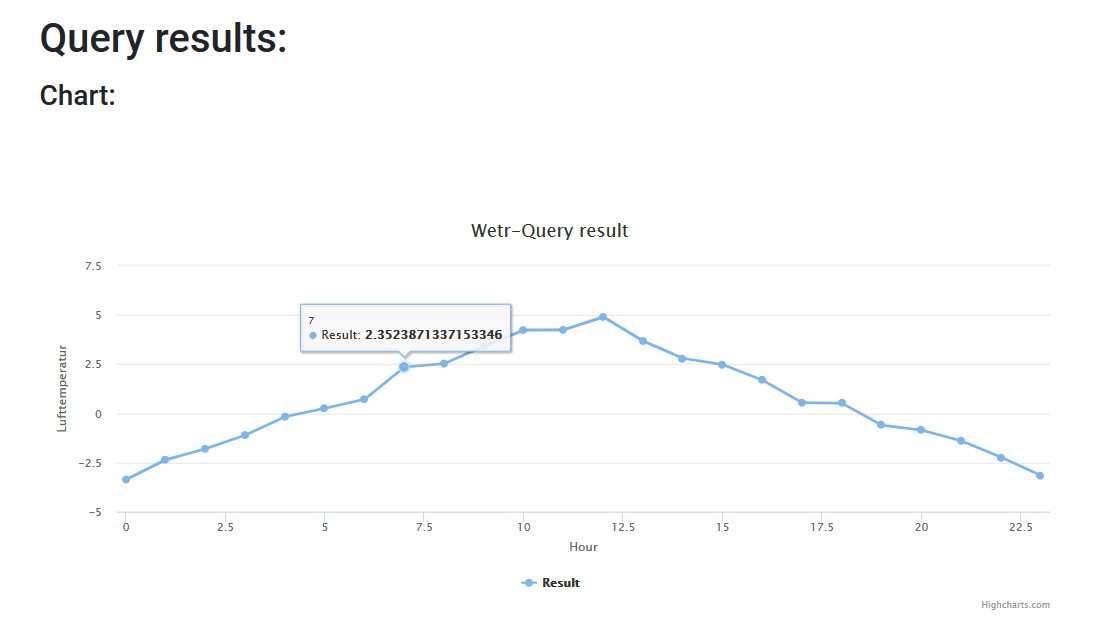
\includegraphics[width=\textwidth]{img/query/query_chart.png}
    \caption{Chart zum Darstellen eines Abfrageergebnisses.}
    \label{fig:query_chart}
\end{figure}

\begin{figure}[H]
    \centering
    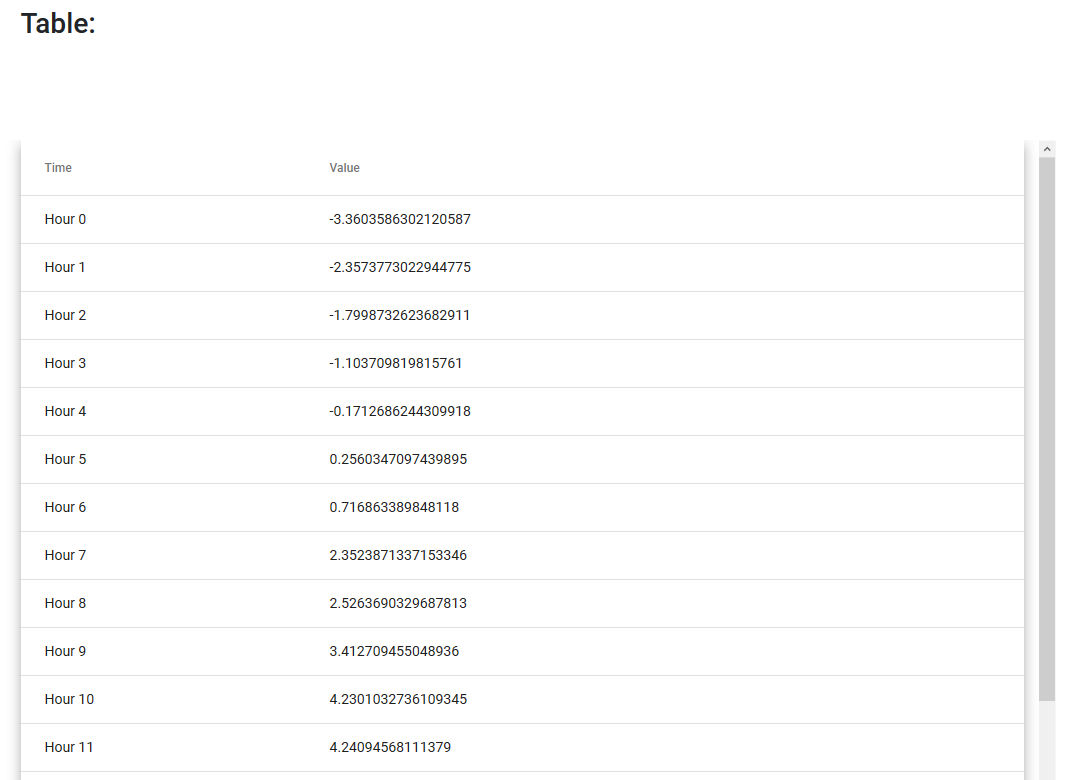
\includegraphics[width=\textwidth]{img/query/query_table.png}
    \caption{Tabelle zum Darstellen eines Abfrageergebnisses.}
    \label{fig:query_table}
\end{figure}

\begin{figure}[H]
    \centering
    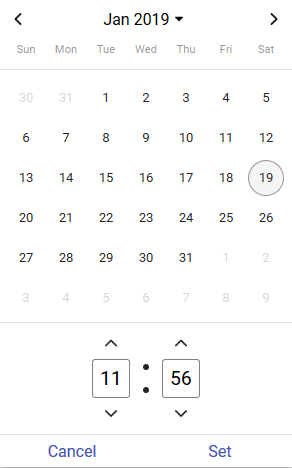
\includegraphics[scale=1.0]{img/query/query_picker.png}
    \caption{DateTimePicker zum auswählen einer Timestamp für das Hinzufügen von Messwerden.}
    \label{fig:query_datetime}
\end{figure}

\newpage

\subsection{Dashboard}

Im Dashboard werden favorisierte Abfragen gespeichert und in Form von DashboardCards angezeigt (Abbildung \ref{fig:dashboard}).
Diese werden pro Benutzer im localStorage gespeichert.
Die genauer Funktionsweise wird in Abschnitt \ref{dashboardcards}) genauer beschrieben.

\begin{figure}[H]
    \centering
    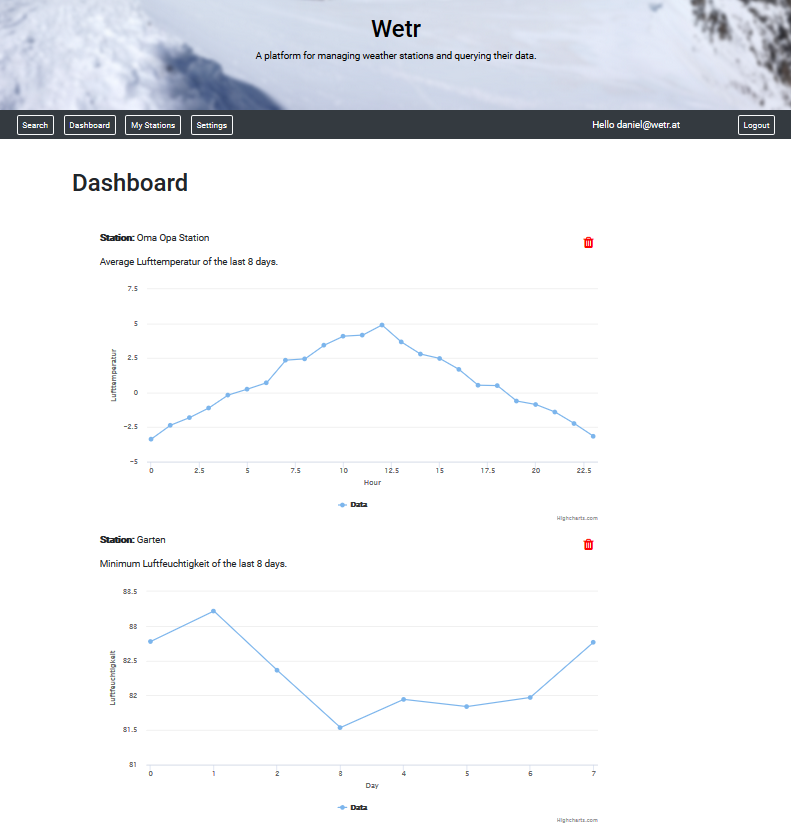
\includegraphics[width=\textwidth]{img/dashboard/dashboard.png}
    \caption{Individuelles Dashboard für den eingeloggten Benutzer.}
    \label{fig:dashboard}
\end{figure}
\newpage

\subsection{DashboardCard}
\label{dashboardcards}

Die DashboardCards können wieder gelöscht werden und zeigen neben den eigentlichen Daten (welche jedes mal neu abgefragt werden) eine kurze Beschreibung an, aus der der Kontext der Daten ersichtlich gemacht werden soll (Abbildung \ref{fig:dashboard_card}). Es können nur Abfragen gespeichert werden die Daten in den letzten X Tagen anzeigen. Somit werden Abfragen deren Zeitraum bereits abgeschlossen ist nicht unterstützt. Das Format der Beschreibung lautet: $<AggragationType>$ $<MeasurementType>$ of the last X days.


\begin{figure}[H]
    \centering
    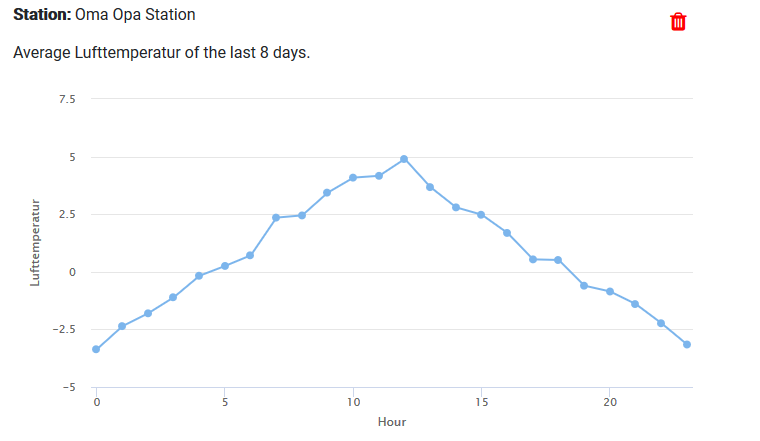
\includegraphics[width=\textwidth]{img/dashboard/dashboard_card.png}
    \caption{Detailansicht einer DashboardCard.}
    \label{fig:dashboard_card}
\end{figure}

\subsection{Settings}

Diese Seite beinhaltet allgemeine Einstellungen, welche im localStorage gespeichert werden (Abbildung \ref{fig:settings}). Beispielhaft gibt es die Einstellung die Temperatureinheit in Fahrenheit zu ändern. Dies wirkt sich auf alle Anzeigen von Temperaturabfragen aus.

\begin{figure}[H]
    \centering
    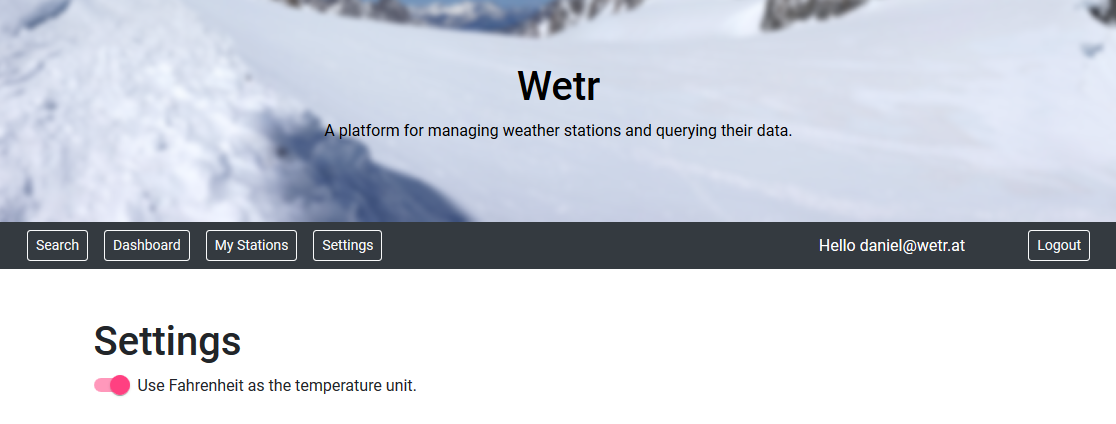
\includegraphics[scale=0.7]{img/settings/settings.png}
    \caption{Settings-Seite.}
    \label{fig:settings}
\end{figure}

\end{document}
